\chapter{OptoTouch DUT applications}
In order to communicate with phones or tablets, a specific DUT application needs to be used. This chapter discusses different DUT applications and their usage.

\section{OptoTouch Android}
OptoTouch Android implements three different functionalities: pen-to-ink (P2I) testing, watchdog (WD) testing, and touch testing. Additionally, it is needed for accurate DUT positioning with both manual and automatic methods. Currently, the latest version of the app cannot be found from app store but it is delivered as APK (android installation package) with the projects.

\tipbox{If touch testing is going to be done, the app should be opened in \emph{pinned mode} if possible. This prevents accidentally swiping any menus open that might prevent the app to function properly.}

\notebox{Remember that the DUT name must be \emph{exactly} the same in the server and the DUT application.}

\begin{wrapfigure}[20]{r}{0.3\linewidth}
	\centering
	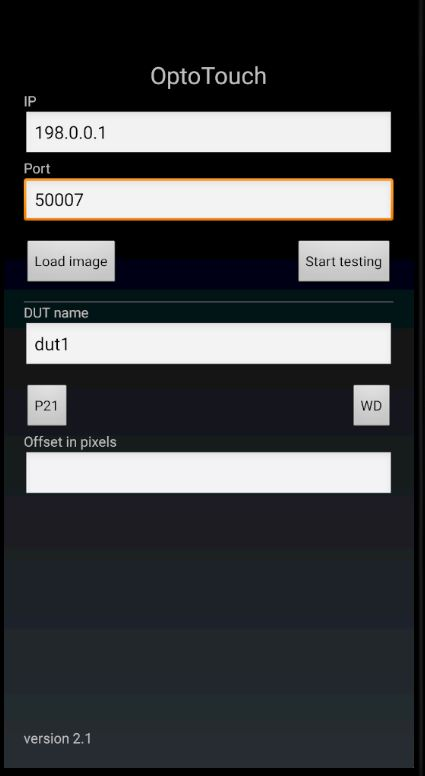
\includegraphics[width=0.8\linewidth]{OptoTouch_Android_main_view.JPG}
	\caption{Main view of OptoTouch Android application.}
	\label{fig:optotouch_android_main}
\end{wrapfigure}

% This text needs to be refined
When app is launched, the main window opens (Fig \ref{fig:optotouch_android_main}). All the functionality can be accessed from the main window. The fields are as follows from top down and right to left:
\begin{itemize}
	\item \texttt{IP:} IP address of the PC the the app is connected. See Subsection \ref{subsec:touch_testing} for more details.
	\item \texttt{Port:} The port to which the app is connected in the PC. See Subsection \ref{subsec:touch_testing} for more details.
	\item \texttt{Load image:} Opens a dialog box for loading an image from DUT memory and shows it on the screen.
	\item \texttt{Start testing:} Connects the DUT to PC for touch testing and automatic positioning. See Subsections \ref{subsec:touch_testing}, \ref{subsec:dut_positioning_features}, and \ref{subsec:communication_with_server} for more details.
	\item \texttt{DUT name:} The name of the DUT given in TnT server. See Subsection \ref{subsec:touch_testing} for more details.
	\item \texttt{P2I:} Opens pen-to-ink measurement view. For more information see \ref{subsec:P2I}
	\item \texttt{WD:} Opens watchdog measurement view. For more information see \ref{subsec:WD}
	\item \texttt{Offset in pixels (deprecated):} Moves the lit corner pixels closer to the screen center in y-axis direction with given amount of pixels. This is a legacy feature for positioning round corner DUTs and not supported in the newer versions of TnT.
\end{itemize}

\subsection{Touch testing}
\label{subsec:touch_testing}
The touch testing view is shown in Figure \ref{fig:touch_testing}. In the upper right corner the device resolution is shown. Below the page header user can see the socket connection statuses. For more information about the socket communication refer to Subsection \ref{subsec:communication_with_server}.

\begin{figure}[h]
	\centering
	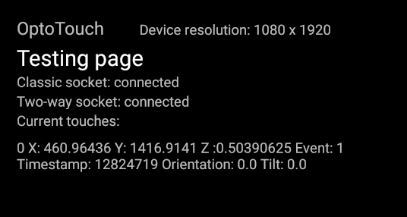
\includegraphics[width=0.7\linewidth]{OptoTouch_Android_touch_testing.jpg}
	\caption{Touch testing view.}
	\label{fig:touch_testing}
\end{figure}

The touch test page also shows the most recent collected touch event data. This information is mainly for debug purposes. The reading showed in the image \ref{fig:touch_testing} tells the following:
\begin{itemize}
	\item \texttt{0:} Touch id given by the operating system to the detected touch. 
	\item \texttt{X:460.96436:} X-coordinate in pixels.
	\item \texttt{Y:1416.9141:} Y-coordinate in pixels.
	\item \texttt{Z:0.50390625:} The pressure number given by the operating system. The exact definition depends on the device and the driver.
	\item \texttt{Event:} The type of touch action that is detected (0 is action down, 1 is action up, and 2 is action move. Basically swipe is something like 0-2-2-2-2-2-2-1)
	\item \texttt{Timestamp:} Androids system uptime in milliseconds.
	\item \texttt{Orientation:} Stylus orientation.
	\item \texttt{Tilt:} Stylus tilt.
\end{itemize}


\subsection{Pen-to-Ink (P2I) testing}
\label{subsec:P2I}
Note that P2I testing requires a HSUP license and special hardware equipment that are not included in a standard delivery.

In the P2I view, the app shows a blank white screen and as the screen is touched, a black line is drawn. When launching this view the user can set the amount of touches that are shown by the black line. The P2I measurement uses high-speed camera to get video image as the robot draws the line and then a machine vision algorithm calculates the latency between finger movement and the end of the drawn line. Refer to Section \ref{sec:HSUP} for more details. 

\subsection{Watchdog (WD) testing}
\label{subsec:WD}
Note that WD testing requires an HSUP license and special hardware equipment that are not included in a standard delivery.

In the WD view, a blank black screen is show and as the screen is touched a white rectangle is shown in the upper right corner of the screen. If the robot finger is equipped with a trigger and a high-speed camera is used, it is possible to measure the touch latency with this view.

\subsection{DUT positioning features}
\label{subsec:dut_positioning_features}
The application supports two modes of positioning:
\begin{enumerate}
	\item \texttt{Manual positioning:} The app main screen has the corner pixels lit with different color than the background. This helps the user focus the positioning camera exactly to the screen corners.
	\item \texttt{Automatic positioning: } Automatic positioning shows a special image on DUT screen that is then recognized with machine vision and used to positioning the DUT. In order to use the automatic positioning, the app has to be in Touch testing mode and two-way socket has to be connected.
\end{enumerate}

\subsection{Communication with server}
\label{subsec:communication_with_server}
The communication between app and server goes through two sockets:
\begin{enumerate}
	\item \texttt{Classic socket:} The app sends constantly all the touch data through this socket and server either collects it or not. On the server side, the classic socket is only opened after TPPT scripts are loaded. On the app side, the classic socket requires the Two-Way socket to be connected. Not having classic socket connection does not prevent the usage of Two-Way socket for e.g. automatic positioning.
	\item \texttt{Two-way socket:} This socket is used for bi-directional communication. Server sends requests and the app replies. This socket is used, for example, to fetch device resolution and send positioning image to the app.
\end{enumerate}


Communication with server is established when the Touch testing mode is entered. The test page shows the statuses of both sockets (see Figure \ref{fig:touch_testing}). The statuses are only updated when the touch testing mode is entered. If the connection is lost it will not reconnect. 

The two parameters (IP address and port) need to be correct in order to have a working connection. The IP address is the one of the measurement PC in the network that connects PC and DUT. The port is basically always 50007 but can be changed. If you need to get the connection through a different port contact OptoFidelity support (more details for that in \ref{part:support})

There are three options to connect the DUT to the server PC:
\begin{enumerate}
	\item \texttt{WiFi:} Connect measurement PC and DUT in the same WiFi network and set the IP address in the app to be the one of the PC in the network. It is also possible to connect the PC directly to the WiFi router with Ethernet cable.
	\item \texttt{USB with tethering:} Connect DUT with USB cable to the measurement PC and enable DUT's network tethering via USB. (DUT does not need to be connected to a network for this.) Then set the IP address in the app to be the one of the PC in the tethered network.  
	\item \texttt{USB with adb (android debug bridge):} Connect DUT to PC via abd and run the following commands.
	\begin{lstlisting}
	> adb reverse tcp:50007 tcp:50007
	> adb reverse tcp:50008 tcp:50008
	\end{lstlisting}
	In the app, set the IP address to be 127.0.0.1.
\end{enumerate}


\section{DUT application troubleshooting}
In this section we have collected the most common issues encountered by our customers. In case you cannot find solution from here contact OptoFidelity support. More information about support can be found from Section \ref{part:support}.

\subsection{Two-way socket not working}
Check that the following things are set correctly:
\begin{itemize}
	\item Check that TnT Server has initialized correctly.
	\item If WiFi connection to PC is used, make sure that PC and DUT are in the same WiFi network or that the PC is connected to the router with Ethernet cable.
	\item Check that the IP address is correct. It is always the PC's address in the network that is used to connect the devices.
	\item Check that the DUT object has been created in TnT Server via e.g. TnT UI and that the DUT name is \emph{exactly} the same in TnT server and DUT app. Also check for accidental whitespace characters.
	\item Check that firewall is not blocking the IP address or port. Try disabling firewall if feasible (the PC should preferably be disconnect from Internet before the disabling). If this fixes the issue, the Firewall settings can then be modified to allow the traffic.
\end{itemize}

\subsection{Classic socket not working}
Check that the Two-way socket is connected and that the TPPT scripts are loaded.

\subsection{App shows that socket is connected but communication is not working}
The socket information is not updated after initialization. Go back in the app by using the DUT's return functionality and tap "Start testing" to get the updated error messages.

\subsection{Connection not working when using USB tethering}
Sometimes when using USB tethering the connection might not work if the ethernet adapter is in DHCP mode. In this case it might help to set a static IP address.